%
\documentclass{aip-cp}

\usepackage[numbers]{natbib}
\usepackage{rotating}
\usepackage{graphicx}
\usepackage{lmodern}
\usepackage[T1]{fontenc}

% Document starts
\begin{document}

% Title portion
\title{Numerical Modeling of Tsunami Propagation on a Sequence of Refining Grids}

\author[aff1]{D.A. Nikiforov}
\eaddress{Corresponding author: m5161111@gmail.com}
\author[aff2]{A.A. Bugaev}
\eaddress{mag@omzg.sscc.ru}
\author[aff1]{A.P. Vazhenin}
\eaddress{vazhenin@u-aizu.ac.jp}

\affil[aff1]{University of Aizu, Tsuruga, Ikki-machi, Aizuwakamatsu, Fukushima,
Japan, 965-8580}
\affil[aff2]{Additional affiliations should be indicated by superscript numbers 2, 3, etc. as shown above.}
%\corresp[cor1]{Corresponding author: m5161111@gmail.com}

\maketitle

\begin{abstract}
The multi-grid algorithm for the tsunami propagation computation from the 
initial source to the coastline that uses scale switching has been 
developed. Computations are carried out on a sequence of grids with various 
resolutions where one is embedded into another. Tsunami wave parameters are 
transferred from a larger domain to the embedded smaller one by means of the 
boundary conditions. Using the method proposed, the numerical simulation of 
tsunami generated by a model ellipsoidal source located in the middle of the 
Pacific was carried out. 
\end{abstract}

% Head 1
\section{INTRODUCTION}
Tsunami sources are usually located in deep-water areas. So, if we want to 
estimate tsunami parameters near the coastline, the computational domain 
must include both a deep and a shallow-water areas. A standard stability 
condition for numerical algorithms used for the modeling requires the wave 
advancement per one time step be less than a spatial grid-step. In this 
case, we should use a small enough time step (for the computation stability 
in deep-water areas of the domain), which makes computations on a shallow 
shelf with an unreasonably small time step be time-consuming. There are a 
number of algorithms and models developed for the tsunami risk mitigation. 
The most known and in general use are TUNAMI \cite{bib1} and MOST (Method
of Splitting Tsunami) [2-4]. These algorithms cover the phases of
generation, propagation of tsunami from the deep ocean to the coastal areas. However, 
the quality of the warning systems is far from being efficient to provide 
the population security. Now it is necessary to develop original algorithms 
for the real time data processing and their adaptation in order to use the 
whole computational power of modern hardware. Modern reliable and fast 
algorithms will contribute to the task of human protection in the shoreline 
areas. The only way to protect people living on the shoreline from 
catastrophic tsunami waves is to make an accurate estimation of expected 
tsunami wave parameters such as height near the shore, wave arrival times, 
etc. 

The numerical modeling of tsunami wave propagation takes much time and 
should be accelerated the sooner the better. Such an acceleration can be 
done with the help of hardware architectures or developing more efficient 
algorithms. The MOST software is used to numerically simulate three 
stages of the tsunami evolution: estimation of a residual displacement 
area resulting from an earthquake and tsunami generation, trans-oceanic 
propagation through deep-water zones, and contact with land (run-up and 
inundation). The given research is concerned with the wave propagation 
stage. 

The rest of the paper is organized as follows. In the next section, the
peculiarities of the shallow-water equations are discussed for the long wave propagation 
over the ocean. Then we are presenting a model of an initial water surface elevation
is presented. Section 4 describes the scaled-switching tsunami modeling
algorithm as well as its comparisons with computation in a whole domain. In
Conclusion we summarize resuts of these investigations. 

%Head 2
\section{THEORETICAL BACKGROUND}
The long wave propagation in the ocean is governed by the so-called 
shallow-water differential equations:

\[
H_t + (uH)_x + (vH)_y = 0,
\]
\begin{equation}
\label{eq1}
u_t + uu_x + vu_y + gH_x = gD_x ,
\end{equation}
\[
v_t + uv_x + vv_y + gH_y = gD_y ,
\]

\noindent
where \textit{H(x, y, t) = h(x, y, t) + D(x, y, t), h} is the water surface displacement, D is depth, u(x, y, t) and v(x, y, 
t) are velocity components along the axes x and y, g is acceleration of 
gravity. The initial conditions: still water at all grid points except a 
tsunami source where a surface displacement is not equal to zero. From the 
shallow-water equations it follows that the tsunami propagation velocity 
does not depend on its length and is expressed by the so-called Lagrange 
formula [2]

\begin{equation}
\label{eq2}
c = \sqrt {g(D + \eta )} .
\end{equation}

This formula plays the key role for the long-wave (tsunami) kinematics. From 
the shallow-water equations the ratio between the running wave height and 
the water flow velocity can be derived. The horizontal flow velocity depends 
on the wave amplitude and water depth

\begin{equation}
\label{eq3}
u = \eta \sqrt {\frac{g}{D}} \quad .
\end{equation}

These relations between tsunami wave parameters are used in the algorithm 
proposed.

The numerical algorithm is based on splitting the difference scheme that 
approximates equations (\ref{eq1}) by spatial directions. A finite difference 
algorithm based on the splitting method has been developed in [2]. To solve 
the shallow wave equations, the splitting method reduces the numerical 
solution with two spatial variables to the solution of two one-dimensional 
equations. It makes possible to use effective finite difference schemes 
developed for one-dimensional problems. Moreover, this method permits one to 
set boundary conditions for a finite difference boundary value problem using 
a characteristic line method. The criterion of stability for the MOST 
algorithm can be written down as 

\begin{equation}
\label{eq4}
\Delta t \le \frac{\Delta x} { \sqrt{gH}} .
\end{equation}

Here $\Delta t$ and $\Delta x$ are the time and the grid steps, respectively. 
This condition requires setting a smaller time step if a computational 
domain contains deep-water areas. For example, if a deep-water trench with a 
depth of 9,000 m is included into the area with 1,000~m resolution 
computational grid, then we must use a 3 sec (or less) time step for the 
stability of computation. At one time step, a tsunami wave must advance a 
distance less than one spatial grid step. In the case of tsunami occurrence, 
a deep-water detector can give the passing tsunami wave parameters 15-20 
minutes after the main shock of a tsunamigenic earthquake. Then a few 
minutes are necessary to obtain the first estimates of the tsunami source 
parameters and its center, in particular, the location of the center (the 
locality of a maximum vertical displacement of the water surface) and a 
value of a maximum vertical elevation. This information allows us to begin 
the numerical calculation of a direct problem of tsunami propagation from 
the source, actually, to the coastline (up to depths of 5-10 m). However, 
for obtaining results of the tsunami propagation, be more reliable 
(distribution of tsunami wave heights in a shelf zone), rather a small step 
of a computational grid (about tens meters) is necessary. If we simulate the 
tsunami propagation in the whole area including both a source zone and sites 
of the coast, we are interested in, using this small spatial grid step, then 
because of the stability condition we will be compelled to carry out 
calculation with a small time step. This will bring about a significant 
increase in the time of numerical calculation that is inadmissible in 
real-time calculations. Therefore it is necessary to carry out such 
calculations with the use of the computational grids whose spatial step 
decreases when approaching the coast.


\section{A MODEL OF ELLIPSOIDAL TSUNAMI SOURCE}
A standard MOST software package uses as an initial water surface elevation 
that is equal to the ocean bottom displacement obtained as a result of 
numerical modeling of the elastic-plastic problem with seismic source with 
specified parameters. In this case, it is not easy to set the initial water 
surface displacement with a specified amplitude at the desired locality. 
However, sometimes it is needed to study the ratio between the initial wave 
height and wave parameters near the coast. In this case it is necessary to 
carry out a number of numerical experiments with specified initial 
parameters. For this purpose two algorithms can be implemented into the MOST 
software package. The first subroutine defines the initial water surface 
displacement having the ellipsoidal shape. Inside this ellipse, the surface 
elevation is expressed by the formula

\begin{equation}
\label{eq5}
H(i,j) = \left( {1 + \cos (\pi \cdot \arg (i,j))} \right) \cdot H_0 ,
\end{equation}

\noindent
where $H_{0}$ is half the water surface displacement at the central point 
($i_{0}$, $j_{0})$ of the ellipse. The parameter \textit{arg(i,j)} gives the ratio between the 
distance to the ellipse center and the distance to the ellipse border in 
this direction

\begin{equation}
\label{eq6}
\arg (i,j) = \left( {\frac{(i - i_0 ) \cdot \cos (\beta ) + (j - j_0 ) \cdot 
\sin (\beta )}{r_1 }} \right)^2 + \left( {\frac{(j - j_0 ) \cdot \cos (\beta 
) - (i - i_0 ) \cdot \sin (\beta )}{r_2 }} \right)^2.
\end{equation}

Here $r_{1}$, $r_{2}$ are the ellipse axis length and \textit{$\beta $} is the long axis 
azimuth. Figure 1 shows the shape of the 2 meters height ellipsoidal source 
with the axes ratio equal to 2 and the water height distribution along the 
ellipse axis.

\begin{figure}[ht]
  \centerline{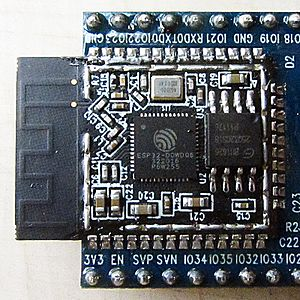
\includegraphics[width=250pt]{art/Fig_01.png}}
  \caption{The shape and cross-section of a model ellipsoidal tsunami source
(The vertical scale is in millimeters)}
\end{figure}

Thus, this subroutine gives the possibility of the numerical simulation of 
the tsunami waves generated by such a kind of sources with a specified 
location and an initial height. Another way to generate a wave with given 
parameters (an amplitude and a wavelength or a period) is to use boundary 
conditions. For example, let at the initial instant of time in the whole 
computational domain the water surface elevation and flow velocity 
components be equal to zero. Then at all the grid points along one boundary 
(for example, left) the following free boundary conditions are fulfilled 
during a limited time period:

\begin{equation}
\label{eq7}
\eta = \frac{\eta _0 }{2}\left( {1 - \cos \left( {\frac{2\pi \cdot t}{T}} 
\right)} \right),
\quad
u = \eta \sqrt {\frac{g}{D}} ,
\end{equation}

\noindent
where \textit{$\eta $}$_{0}$ is a wave height and $T$ is its period, $g$ is the gravity 
acceleration, $D$ is the depth. As a result, the flat tsunami wave having the 
amplitude \textit{$\eta $}$_{0}$ and the period T will propagate from this left boundary 
inside the computational domain.

\section{MULTI-GRID COMPUTATIONS OF THE TSUNAMI WAVE PROPAGATION}

We propose the algorithm, which consists in a consecutive calculation of the 
tsunami wave propagation in several computational domains, where each 
subsequent computational area is a subarea to the previous one, but with a 
smaller spatial step. And initially in these subareas there is no tsunami 
source (the initial vertical water surface displacement). Information on 
parameters of a wave is transferred to each subsequent subarea through 
boundary conditions, thus these data are interpolated along the boundary on 
a smaller computational grid. 

\subsection{Nested Computational Domains}
Digital bathymetry sets were taken or 
developed using different sources. The first stage of the numerical 
simulation uses the whole-Pacific gridded bathymetry developed by Smith and 
Sandwell [5], which is now used by the NOAA for the trans-pacific tsunami 
modeling. The limits of this computational domain are shown in Figure 2.

\begin{figure}[h]
  \centerline{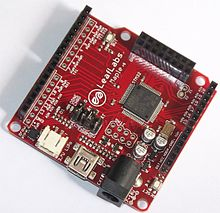
\includegraphics[width=250pt]{art/Fig_02.png}}
  \caption{The coverage of the whole Pacific computational domain (B0 area).}
\end{figure}

Resolution of this digital bathymetry is varying from 4 arc minutes (about 
8,000 m) at the equator to 2 arc minutes (approx. 4,000 m) closer to the 
polar areas. The geographic coverage of these data (area B0) is from 
120$^{o}$ E to 68$^{o}$ W and from 73.96$^{o}$ S up to 62$^{o}$ N.

For further stages of the modeling, the area of the Pacific Ocean adjacent 
to the northwest of the island of Honshu (Japan) is chosen. The gridded 
digital bathymetry for the numerical modeling was developed using 500 m 
resolution bathymetry around Japan [6] (\underline 
{\textit{http://jdoss1.jodc.go.jp/cgi-bin/1997/depth500{\_}file}}) by 
recalculating the depth to the geographical projection grid and 1 
arc sec ASTER Global digital elevation model [7] (\underline 
{http://www.gdem.aster.ersdac.or.jp/search.jsp}).

The size of a computational rectangular grid, in which knots preset values 
of a depth was taken as 1,610$\times$1,610 knots. The length of a spatial step in 
both directions is equal to 0.0049688 geographical degrees that is about 550 
meters in the South-North direction and about 440 m in the West-East 
direction. The bottom topography of this computational domain B1, stretching 
from 34 to 40 degrees North Latitude and from 140 to 146 degrees East 
Longitude, is shown in Figure 3.

\begin{figure}[h]
  \centerline{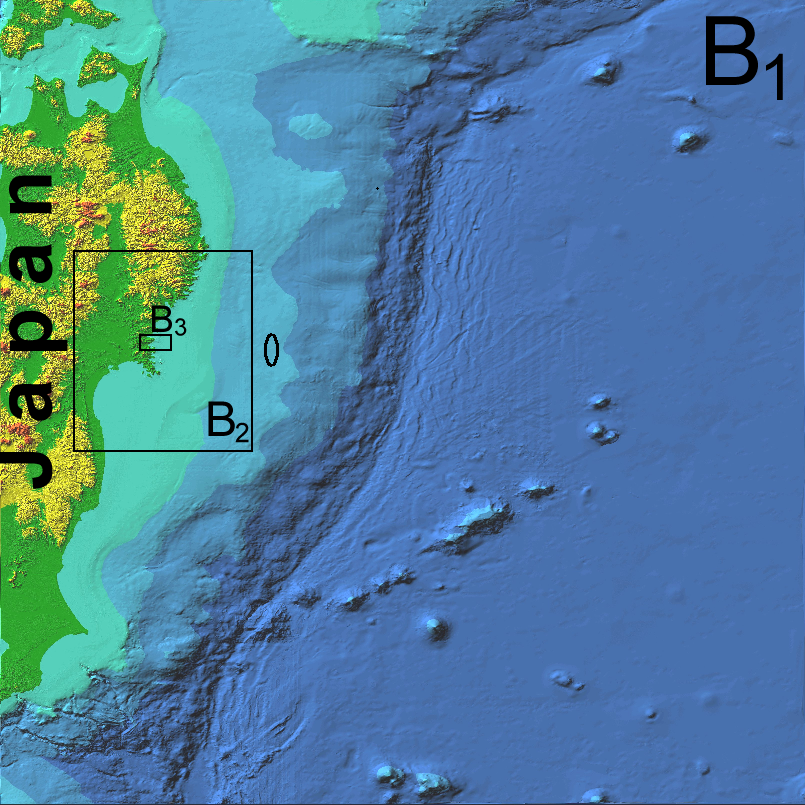
\includegraphics[width=250pt]{art/Fig_03_2.png}}
  \caption{Visualization of the 1,610$\times$1,610 gridded bottom relief around the 
NE coast of the Honshu island. The mesh size: 0.00496$\times$0.00496 arc degrees 
(442$\times$554 m).}
\end{figure}

The location of B1 computational domain inside B0 area is shown in Figure 2. 
The B1 grid covers the geographic area from 140$^{o}$ to 147.9944 $^{o}$ E 
and from 34.00$^{o}$ up to 41.9948$^{o}$ N. At the third stage of the 
numerical experiment, the 2,797$\times$3,197 knots computational grid (B2), which 
covers the part of the Tohoku shelf area, was used. These data were 
developed with a linear interpolation from a segment of the B1 computational 
area. B2 grid covers the area from 140.745$^{o}$ E to 142.48$^{o}$ E and 
from 37.53$^{o}$ N up to 39.51$^{o}$ N. The Grid resolution of the B2 area 
was taken 8 times less than in the B1 computational area and being equal to 
0.0006211 arc degrees. At the final stage of the computational experiment, 
the tsunami wave entering the Sanriku coast harbors was studied. The gridded 
bathymetry of this small area was developed using a detailed (scale 
1:50,000) raster bathymetric chart of the Oppa and the neighboring harbors 
(Figure 4).

\begin{figure}[h]
  \centerline{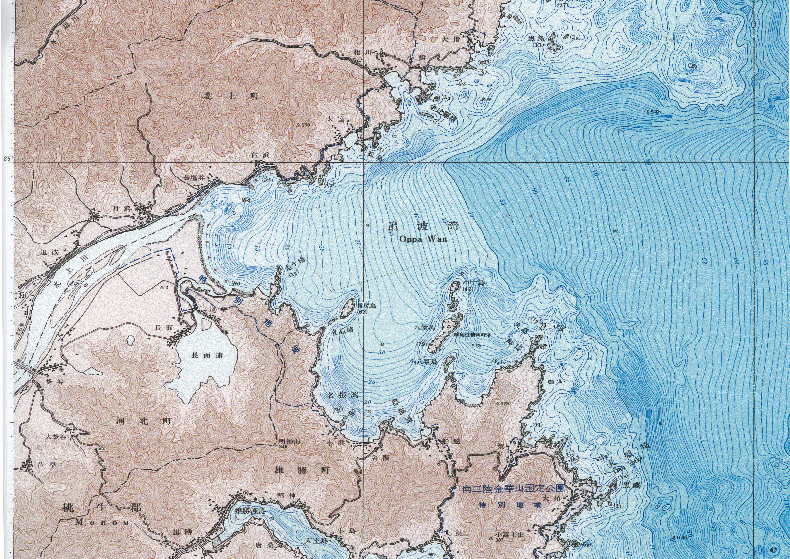
\includegraphics[width=300pt]{art/Fig_04.png}}
  \caption{The scan of the bathymetric chart that was used for developing a 
gridded bathymetry (scale factor 1:50,000)}
\end{figure}

Using the Global Mapper software the isolines of a depth in the bottom part 
of Figure 4 were digitized. Then the 1 arc sec resolution ASTER GDEM digital 
relief [7] was added, and with the help of the Global Mapper software these 
data were interpolated into the gridded digital bottom relief (Figure 5).

\begin{figure}[h]
  \centerline{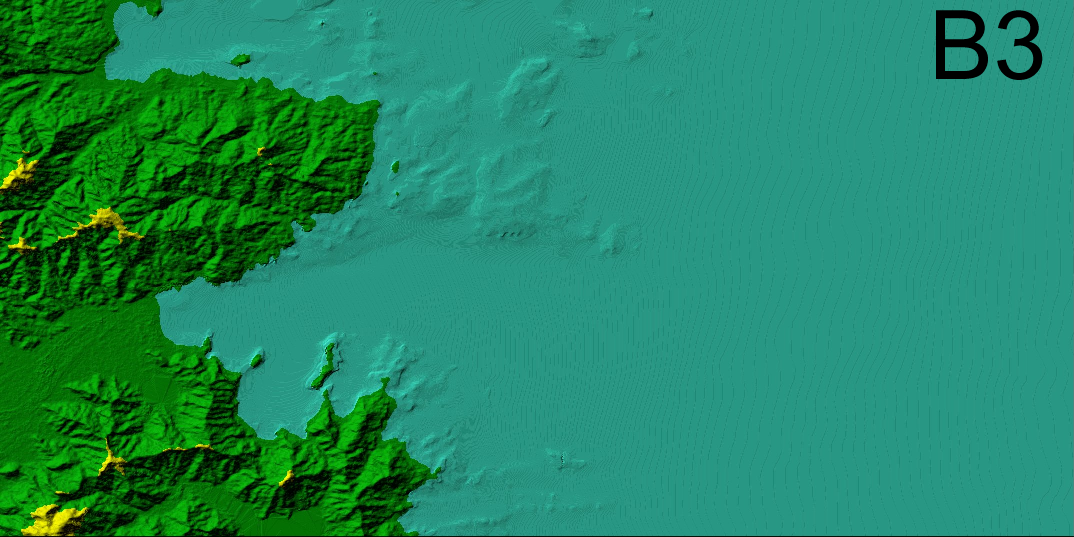
\includegraphics[width=300pt]{art/Fig_05.png}}
  \caption{Visualization of the Oppa harbor bottom topography}
\end{figure}

As a result, the 2148x1074 knots gridded bathymetry for the Oppa and the 
neighboring harbors was created (B3 computational domain). The length of a 
grid step is equal to 0.000155275 arc deg (approximately 17 m). These data 
cover the geographical area from 141.41659$^{o}$ E to 141.75$^{o}$ E and 
from 38.5$^{o}$ N up to 38.6666$^{o}$ N. The spatial step of the grid here 
is 4 times smaller than in B2 computational area. The location of B2 and B3 
computational domains inside the B1 area is shown in Figure 3.

The summary of these four computational grids is as follows:


B0 is the gridded 2581$\times$2879 knots computational area with aprox. 4 
arc-minute resolution (about 5,000 m). The time step for computations is 
equal to 4 sec.


B1 is the gridded 1610$\times$1610 knots computational area with 0.00496 arc-degree 
resolution (about 560 m). The time step for computations is equal to 0.5 
sec.


B2 is the gridded 2797$\times$3197 knots computational area with 0.000621 
arc-degree resolution (about 70 m). The time step for computations is equal 
to 0.5 sec.


B3 is the gridded 2148$\times$1074 knots computational area with 0.000155 
arc-degree resolution (about 17 m). The time step for computations is equal 
to 0.25 sec.


\subsection{Scale-switching tsunami modeling}
At the first stage of the simulation, the process of tsunami generation by 
the ellipsoidal initial ocean surface displacement (Figure 1) and the 
following wave propagation in a deep ocean was carried out. The model 
tsunami source of the ellipsoidal shape is located not far from the right 
border of the computational subarea B1. The axis length taken was 210 km in 
the vertical direction and 70 km -- in the horizontal (Figure 6a). The level 
elevation value at the source center was equal to 200 cm. The distance off 
B1 computational area boundary was chosen sufficiently small in order not to 
wait too long for the tsunami arrival to this boundary. Figure 6a presents a 
zoomed segment of B0 area with the initial tsunami source. 

\begin{figure}[h!]
 \hspace*{3mm}
 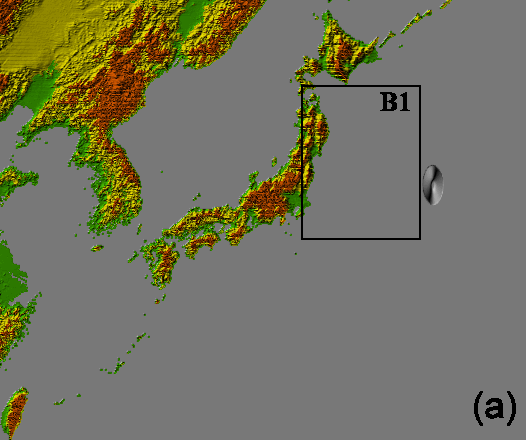
\includegraphics[width=8cm,height=8cm]{art/Fig_06_a.png}
 \hfill
 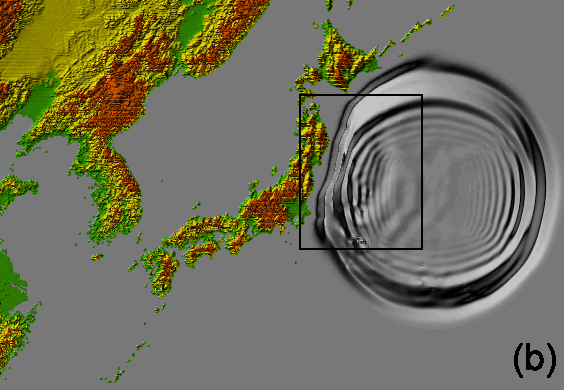
\includegraphics[width=8cm,height=8cm]{art/Fig_06_b.png} \hspace*{3mm}
\\
\parbox[t]{0.45\textwidth}{\caption{The ocean surface of the domain B0
at two istants of time}} \hfill
\end{figure}


In Figures 6 (a)-(b), the ocean surface at several instants of time is visualized. 
The black rectangle shows the B1 area boundary location. 

At the first stage of the numerical experiment, the wave propagation in the 
``large'' computational domain B0 almost up to the coast of Japan was 
simulated. The time step for this computation was equal to 4 sec. In the 
whole process of computation, the wave parameters (amplitude, horizontal 
velocity components and geographical coordinates) at all the grid points 
along B1-area boundaries were output into a file. The data output starts 
from the very first time step and continues at every time step. Data 
recording can be stopped when a tsunami wave has passed the right boundary 
of the subarea B1$_{ }$(at least the whole wave period). The gridded 
bathymetries of computational areas B0 and B1 are not well correlated. This 
means that there are almost no grid points having same geographic location. 
As was already noticed the grid-step length in these two areas significantly 
differs (about 5,000 meters against approximately 560 m). Let us take one 
column of B0 area grid points which are most closely situated to the right 
vertical boundary of B1. The latitudes of these B0 domain grid points are 
saved in 1D array \textit{lat0(i), i=1,N}. Using the linear interpolation the tsunami wave 
parameters at B1 boundary grid-points with the latitudes lat1(j), j=1,M are 
being calculated.

\begin{figure}[h!]
 \hspace*{3mm}
 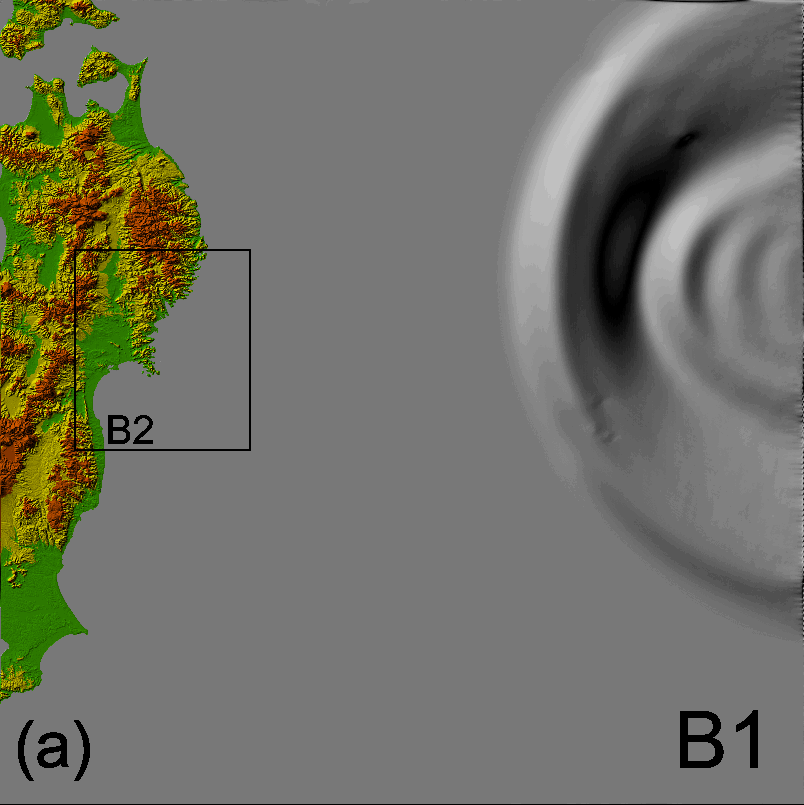
\includegraphics[width=7cm,height=7cm]{art/Fig_07_a.png}
 \hfill
 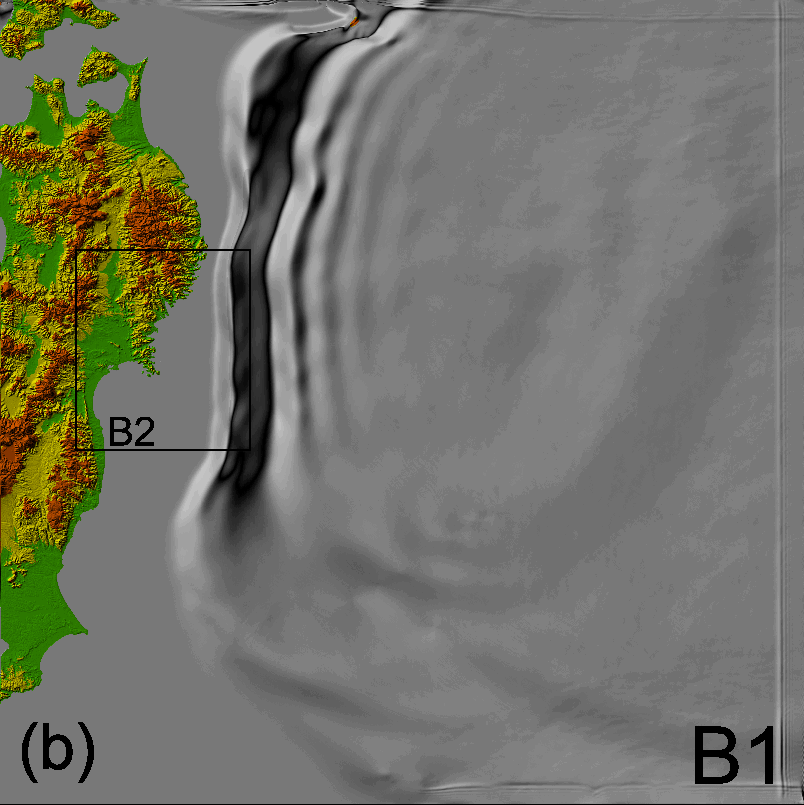
\includegraphics[width=7cm,height=7cm]{art/Fig_07_b.png} \hspace*{3mm}
\\
\parbox[t]{0.45\textwidth}{\caption{Visualization of the wave 
propagation at the B1 subarea}} \hfill
\end{figure}


The formulas for recalculating the wave parameters along the B1 domain 
boundary are as follows:


\[
\eta 1(j) = \left( {\eta 0(i + 1) \cdot (lat1(j) - lat0(i)) + \eta 0(i) 
\cdot (lat0(i + 1) - lat1(j))} \right) / (lat0(i + 1) - lat0(i)),
\]


\[
u1(j) = \sqrt {\frac{D0(i)}{D1(j)}} \left( {u0(i + 1) \cdot (lat1(j) - 
lat0(i)) + u0(i) \cdot (lat0(i + 1) - lat1(j))} \right) / (lat0(i + 1) - 
lat0(i)).
\]


Here the parameters \textit{$\eta $0(i), u0(i)} are related to the B0 computational area and \textit{$\eta $1(j), u1(j)} are 
related to B1 area. If time steps are different, then wave parameters must 
also be interpolated with respect to time. Thus, after recalculating the 
flow parameters along B1 boundaries the second stage of the numerical 
experiment can be started. In this computational area, the boundary value 
problem is solved. The ocean surface elevation at several instants of time 
is visualized in Figures 7a-7b.


In the course of computations in the area B1, the flow parameters values 
along the boundaries are to be read at every time step and the flow 
parameters along B2 subarea boundaries (Figure 3) being a result of the 
numerical computation are also to be saved in the new text file 
``bound{\_}2.dat''. 

After finishing the numerical simulation of the tsunami propagation in B1 
computational domain the boundary data from the file ``bound{\_}2.dat'' are 
to be recalculated to a more detailed grid with the help of linear 
interpolation. Then the third stage of the numerical experiment is ready to 
be started. As was performed at the previous stages, the boundary value 
problem in B2 area is being numerically solved. The results of this 
simulation are presented in Figures 8a-8b.

\begin{figure}[h!]
 \hspace*{3mm}
 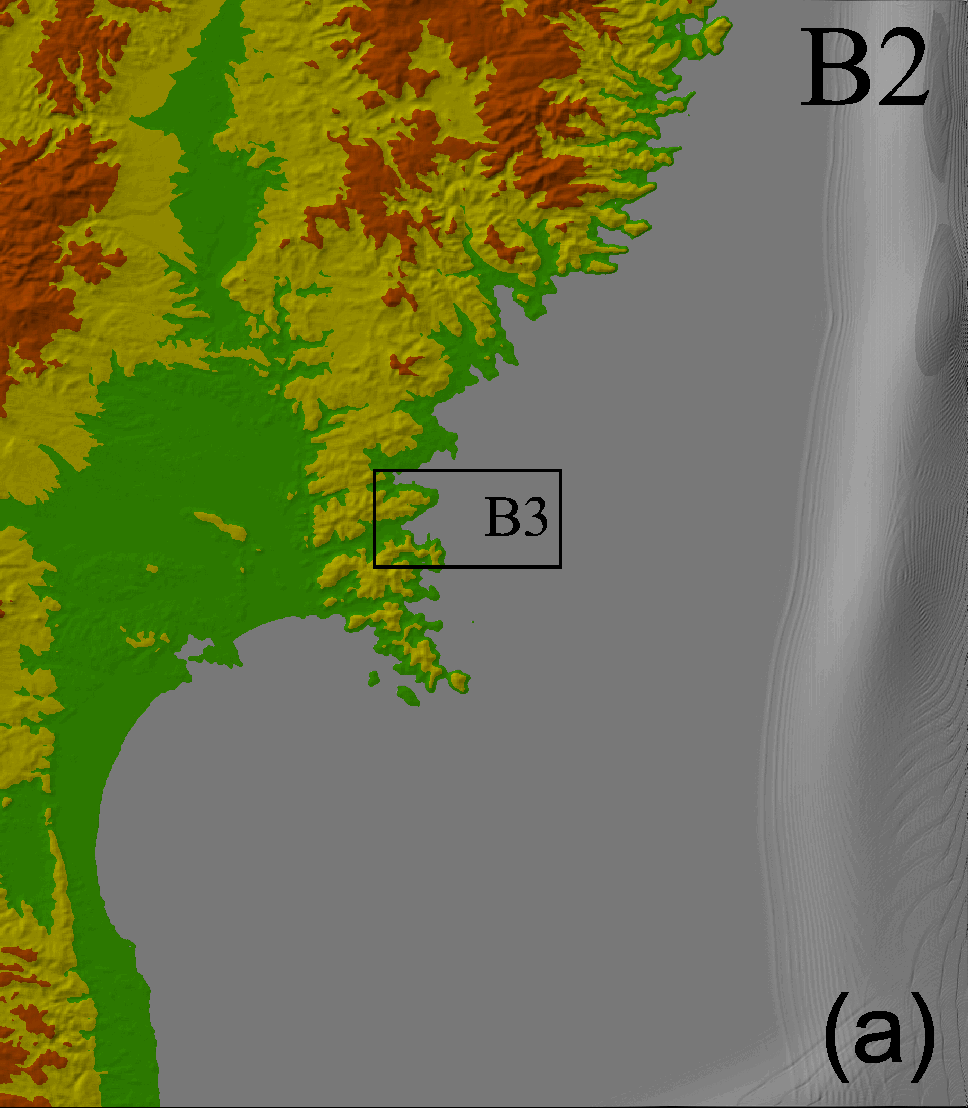
\includegraphics[width=7cm,height=9cm]{art/Fig_08_a.png}
 \hfill
 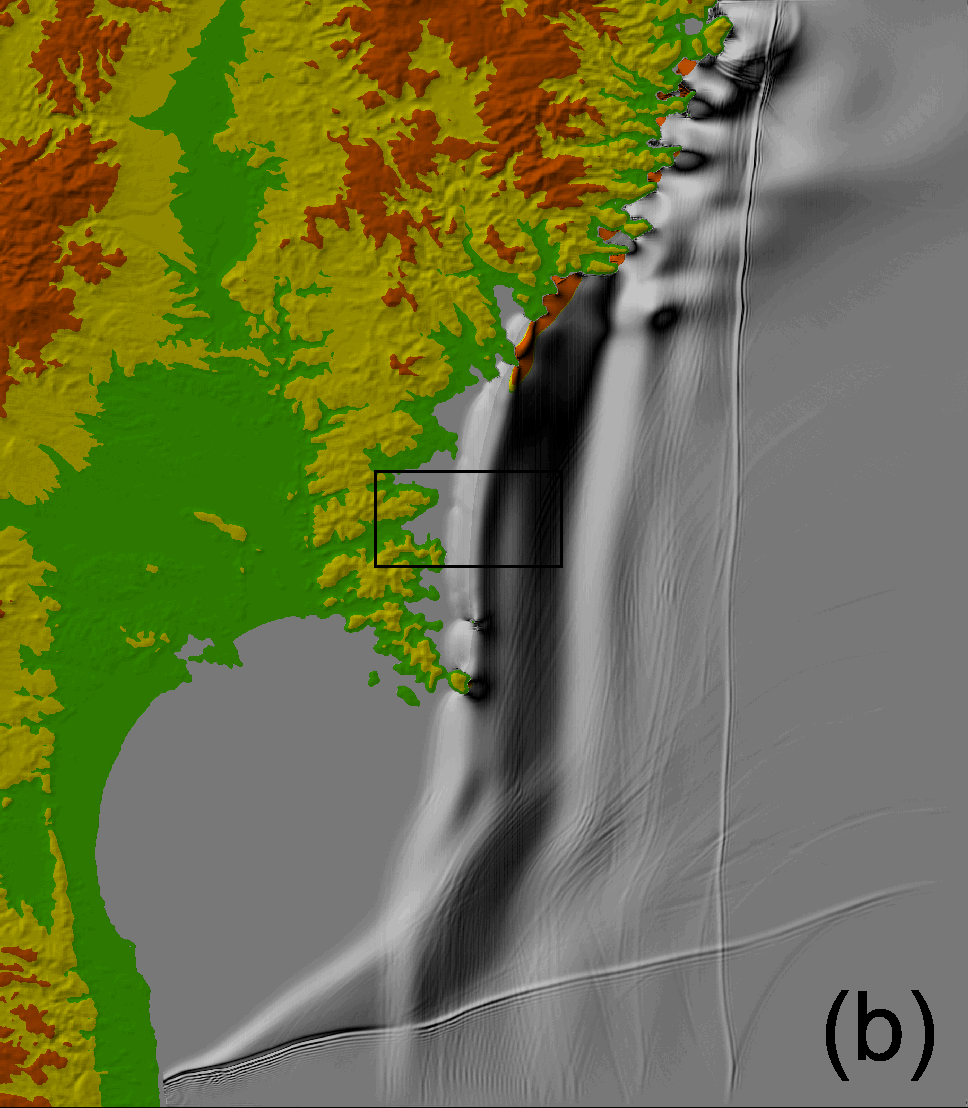
\includegraphics[width=7cm,height=9cm]{art/Fig_08_b.png} \hspace*{3mm}
\\
\parbox[t]{0.45\textwidth}{\caption{The result of tsunami 
propagation through the B2 domain}} \hfill
\end{figure}


As was done at the previous stage of this numerical experiment, the new data 
file ``bound{\_}3.dat'' containing the wave parameters along the boundaries 
of B3 computation subarea was created. Then, as usual, these data are to be 
recalculated to a more detailed grid that will be used in B3 computational 
domain. Due to the fact that the fourth stage of the numerical experiment is 
declared as the last one, no boundary data are to be saved in computations 
in the B3 area. The results of the numerical modeling near the Sanriku coast 
and inside the Oppa harbor are presented in Figures 9-10.

\begin{figure}[h]
  \centerline{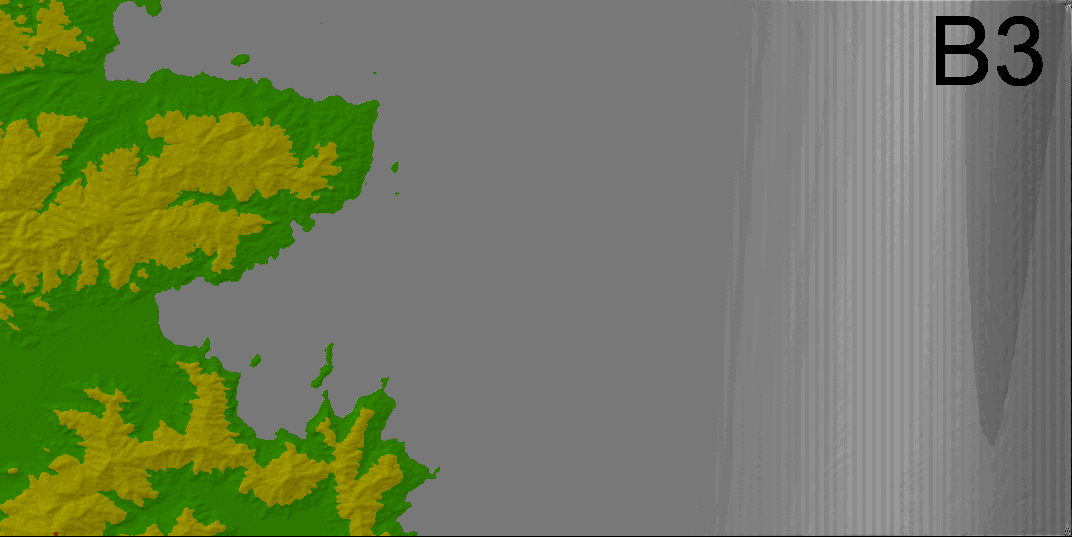
\includegraphics[width=300pt]{art/Fig_09.png}}
  \caption{}
\end{figure}

\begin{figure}[h]
  \centerline{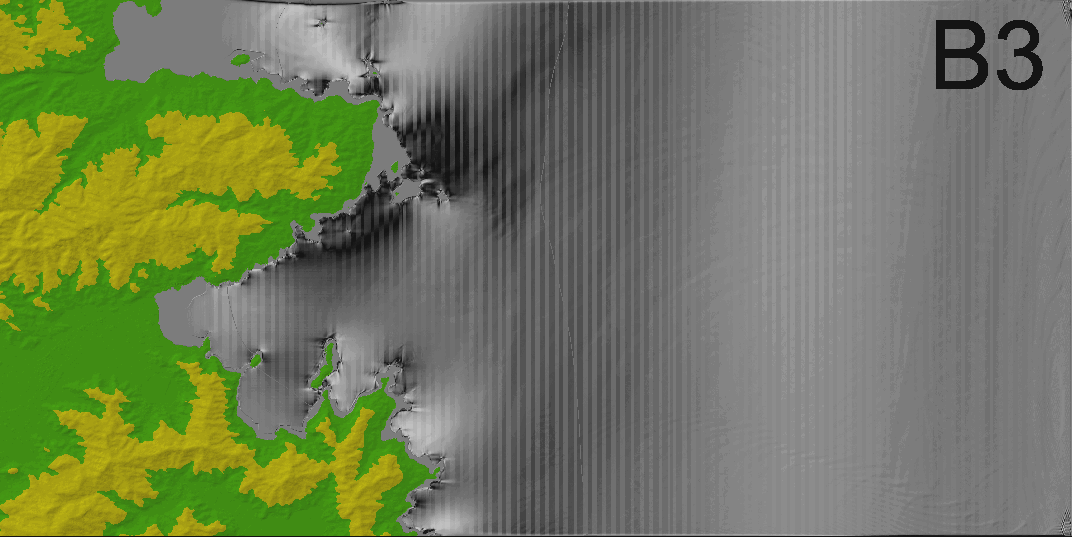
\includegraphics[width=300pt]{art/Fig_10.png}}
  \caption{}
\end{figure}

Thus, a sequence of actions which we call ``the multi-grid algorithm for the 
numerical modeling of tsunami propagation'' is described and shown on an 
example. Using this algorithm, the influence of a wavelength and resolution 
of computational grids on the tsunami height near the coastline was studied. 
The process of tsunami wave propagation generated by two model ellipsoidal 
tsunami sources having a different size was numerically computed. Each case 
was simulated using a ``rough'' grid (270 m). Then computations use grid 
switching from a ``rough'' to an ``intermediate'' (approx. 70 m) grid. And, 
finally, the numerical experiment was carried on with the help of the 
3-stage multi-grid algorithm (B1, B2 and B3 domains). These numerical 
experiments were carried out for the model ellipsoidal sources that generate 
a tsunami having period 200 and 500 sec (``small'' and ``large'' sources situated inside B1 area). 
Let us consider the first case (a shorter wave). Figure 11a presents the 
water surface inside the Oppa harbor as a result of the numerical modeling 
using B1 computational grid. Another picture (Figure 11b) shows the results 
obtained in the same geographic area at the same instant of time using 
2-stage grid switching (from B1 to B2 grids). Figure 12a shows a zoomed segment 
of Figure 11b. Figure 12b presents the results of numerical computations of 
the same problem (propagation of the tsunami generated by a ``small'' 
ellipsoidal source using 3-stage grid switching. 

\begin{figure}[h!]
 \hspace*{3mm}
 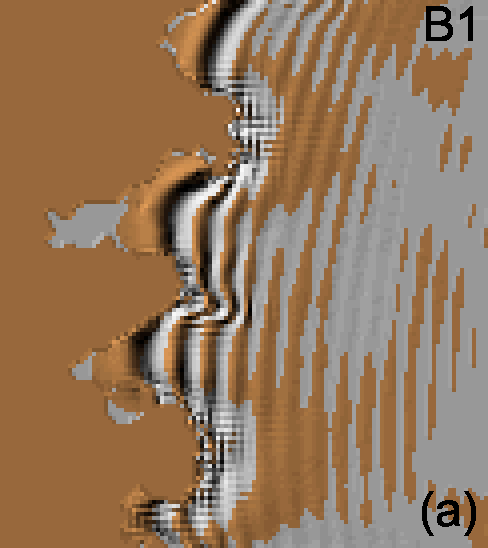
\includegraphics[width=7cm,height=9cm]{art/Fig_11_a.png}
 \hfill
 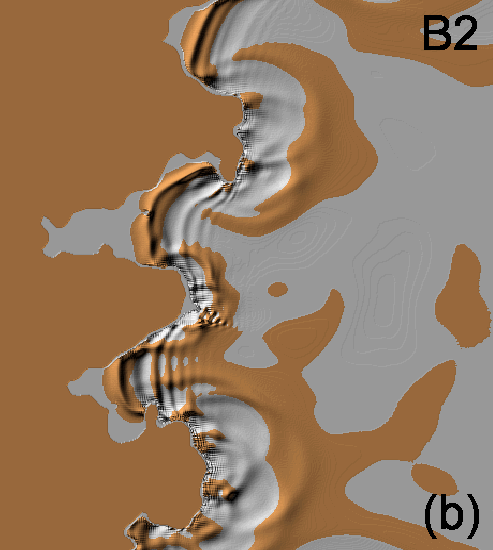
\includegraphics[width=7cm,height=9cm]{art/Fig_11_b.png} \hspace*{3mm}
\\
\parbox[t]{0.45\textwidth}{\caption{}} \hfill
\end{figure}


\begin{figure}[ht]
  \centerline{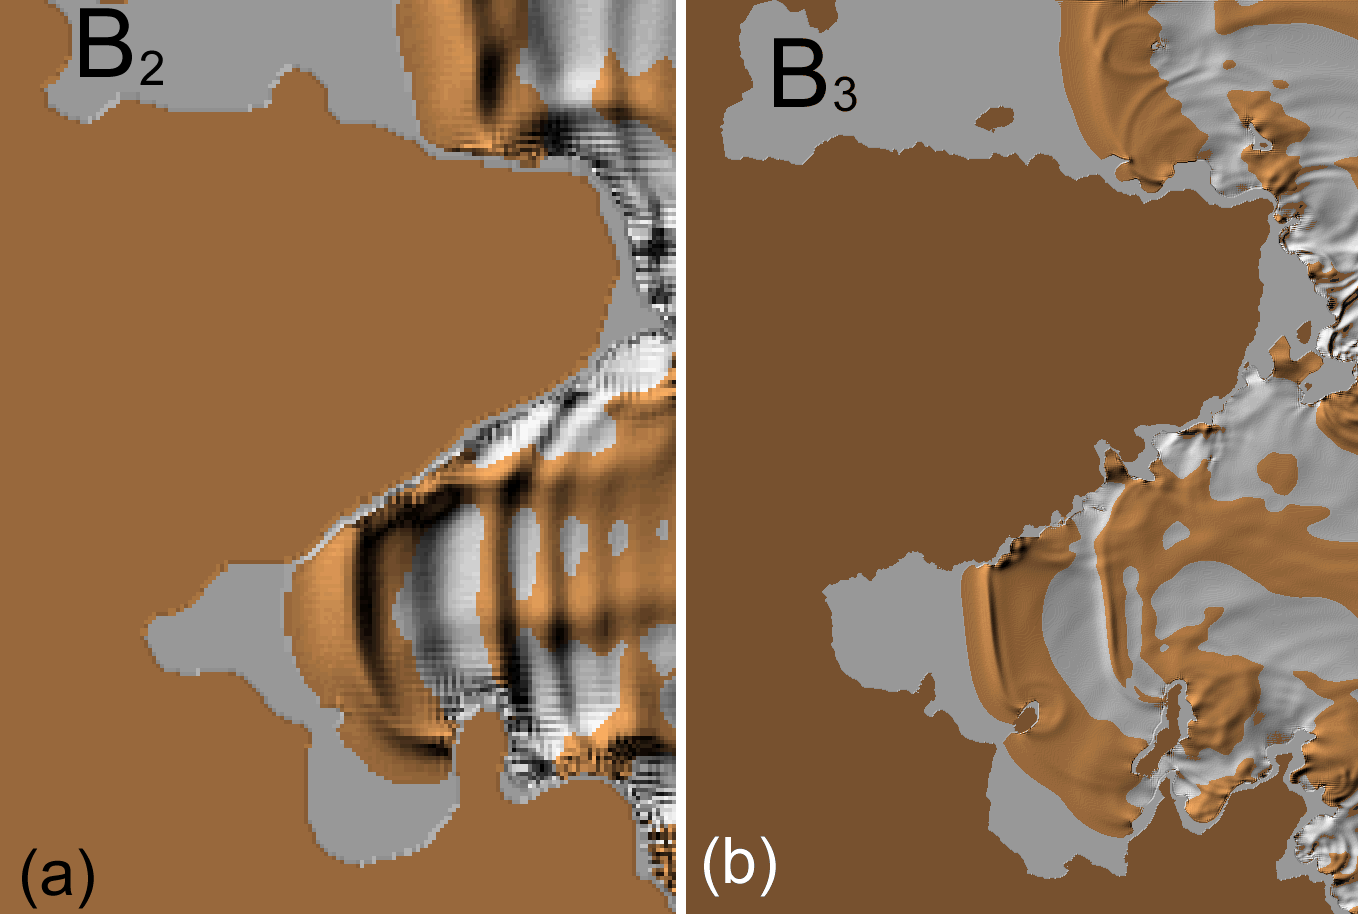
\includegraphics[width=400pt]{art/Fig_12_ab.png}}
  \caption{Comparison of the ocean surface inside Oppa harbor obtained with different grids}
\end{figure}


\subsection{Comparison with a whole computation domain}
The comparison of tsunami parameters near the shore (in the harbors) shows a 
much better quality of the tsunami simulation using the scale-switching 
computations (Figure 11b) as compared to the results of modeling on B1 
(Figure 11a). Also, a significant difference between 
the two-grid and the three-grid numerical experiments can be easily seen. It 
is clear that on the rough computational grid, the wave in harbors is 
longer. Its amplitude is lower and it is much more reflected off the 
near-costal bottom slope (Figures 12a and 12b). A similar trend is seen when the 
``long'' wave propagates through B1-B2-B3 computational areas. Here we give 
the summary of the detected leading wave height inside the Oppa harbor (Figure 13).

The wave period=200 sec:

B1 grid: h=0.5 m

B2 grid: h=1.5 m

B3 grid: h=1.9 m

The wave period=500 sec:

B1 grid: h=0.9 m

B2 grid: h=1.6 m

B3 grid: h=1.9 m

\begin{figure}[h]
  \centerline{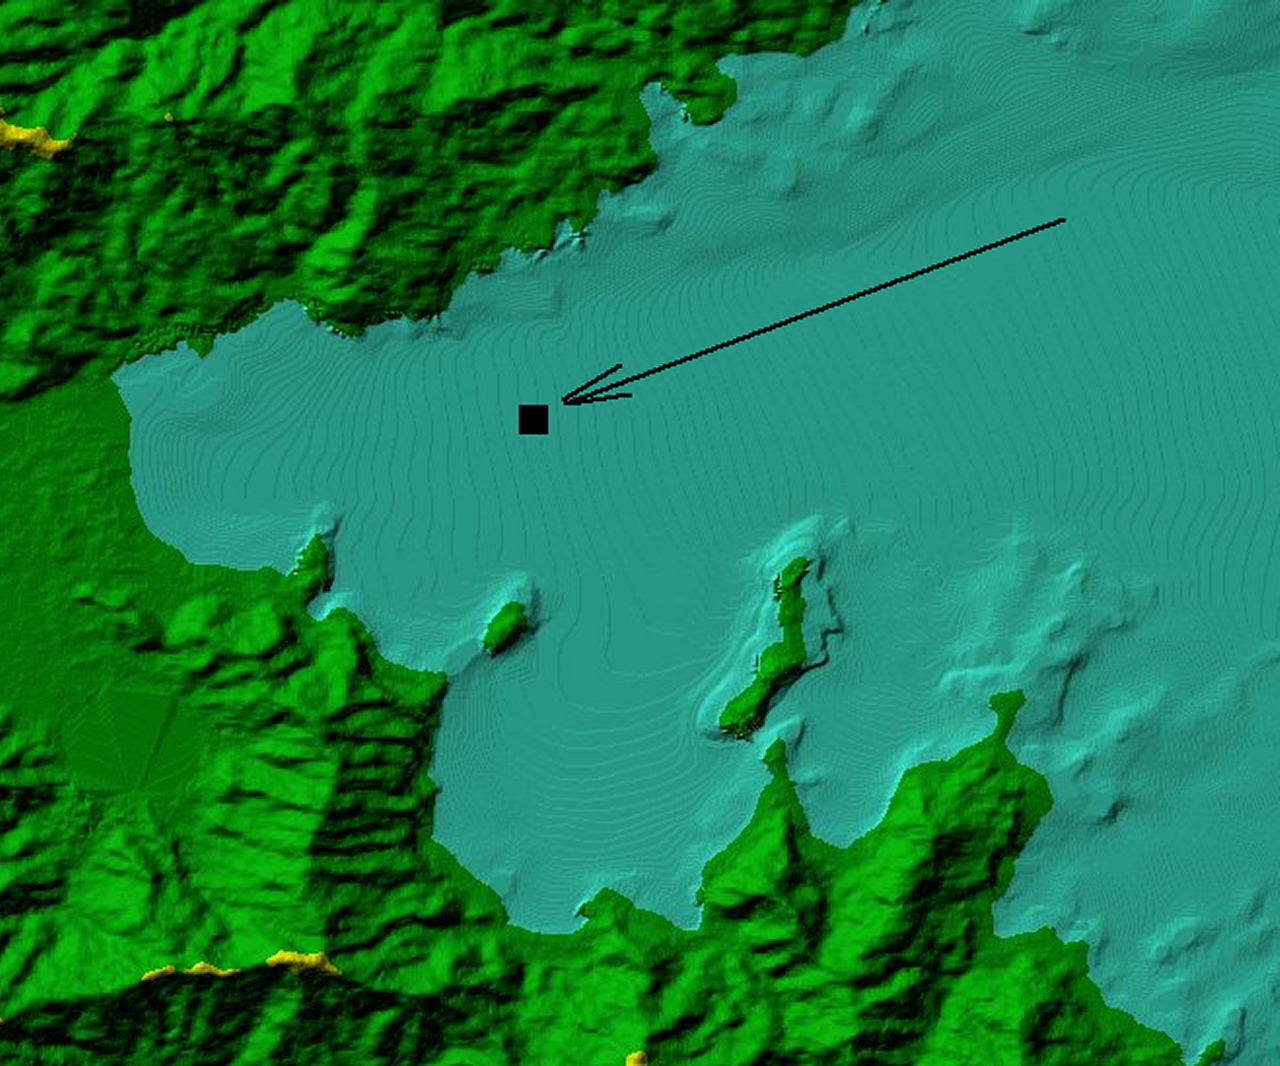
\includegraphics[width=300pt]{art/Fig_13.png}}
  \caption{Location of the data output inside the Oppa harbor}
\end{figure}

These data show that for a shorter tsunami wave the effect of using the 
multi-grid algorithm is greater than that for long tsunami waves (a period 
greater than 8 minutes).

\section{CONCLUSION}

Computational grids must have different spatial resolutions when modeling 
tsunami propagation in the deep ocean and on the shallow shelf.

Tsunami wave parameters can be transmitted from a larger domain to the 
embedded smaller one by means of boundary conditions.

The method proposed effectively works in the case of poor correlated gridded 
bathymetries with different resolutions.

The method was implemented into the standard MOST software and tested on the 
tsunami propagation modeling in the areas with a real bathymetry around 
Japan. 



% Sections that will go in second font

% Acknowledgement
\section{ACKNOWLEDGMENTS}
This work is supported by the Grand-In-Aid for Scientific Research (Ba- sic), 2015-2017, Japan, Issue Number: 15K00103.

% References

\nocite{*}
\bibliographystyle{aipnum-cp}%
\bibliography{ref}%


\end{document}
